\documentclass{article}

\usepackage[margin=1in]{geometry} 
\usepackage{amsmath,amsthm,amssymb}
\usepackage{graphicx}
\usepackage{tikz}
\usepackage{pgfplots}
\pgfplotsset{compat=newest}

\newcommand{\R}{\mathbb{R}}
\newcommand{\Z}{\mathbb{Z}}
\newcommand{\N}{\mathbb{N}}
\newcommand{\Q}{\mathbb{Q}}
\newcommand{\C}{\mathbb{C}}

\newenvironment{theorem}[2][Ejercicio]{\begin{trivlist}
\item[\hskip \labelsep {\bfseries #1}\hskip \labelsep {\bfseries #2.}]}{\end{trivlist}}
\newenvironment{lemma}[2][Lemma]{\begin{trivlist}
\item[\hskip \labelsep {\bfseries #1}\hskip \labelsep {\bfseries #2.}]}{\end{trivlist}}
\newenvironment{exercise}[2][Exercise]{\begin{trivlist}
\item[\hskip \labelsep {\bfseries #1}\hskip \labelsep {\bfseries #2.}]}{\end{trivlist}}
\newenvironment{problem}[2][Problem]{\begin{trivlist}
\item[\hskip \labelsep {\bfseries #1}\hskip \labelsep {\bfseries #2.}]}{\end{trivlist}}
\newenvironment{question}[2][Question]{\begin{trivlist}
\item[\hskip \labelsep {\bfseries #1}\hskip \labelsep {\bfseries #2.}]}{\end{trivlist}}
\newenvironment{corollary}[2][Corollary]{\begin{trivlist}
\item[\hskip \labelsep {\bfseries #1}\hskip \labelsep {\bfseries #2.}]}{\end{trivlist}}

\newenvironment{solution}{\begin{proof}[Solution]}{\end{proof}}

\begin{document}

\title{Métodos Numéricos de Optimización con restricciones.}
\author{Bustos Jordi\\Práctica II}

\maketitle

\section*{Sección 3.2}
\begin{theorem}{1}
    Sean \(f : \mathbb{R}^n \to \mathbb{R}, x, d \in \mathbb{R}^n, \lambda > 0\) tales que
    \(x + \lambda d\) cumple la condición de Armijo. Sea \(0 < \mu < \lambda \).
    ¿Cumple \(\mu \) la condición de Armijo? Pruébelo o dé un contraejemplo que puede ser gráfico.
\end{theorem}

\begin{proof}
    Análogamente al ejemplo visto en clase podemos ver que no siempre se cumple la condición de Armijo para \( 0 < \mu < \lambda \) pues en este caso, si
    \( \mu \in (x_1, x_2) \) no se cumple la regla de armijo y sin embargo se vale que \( \mu < \lambda \). \\
    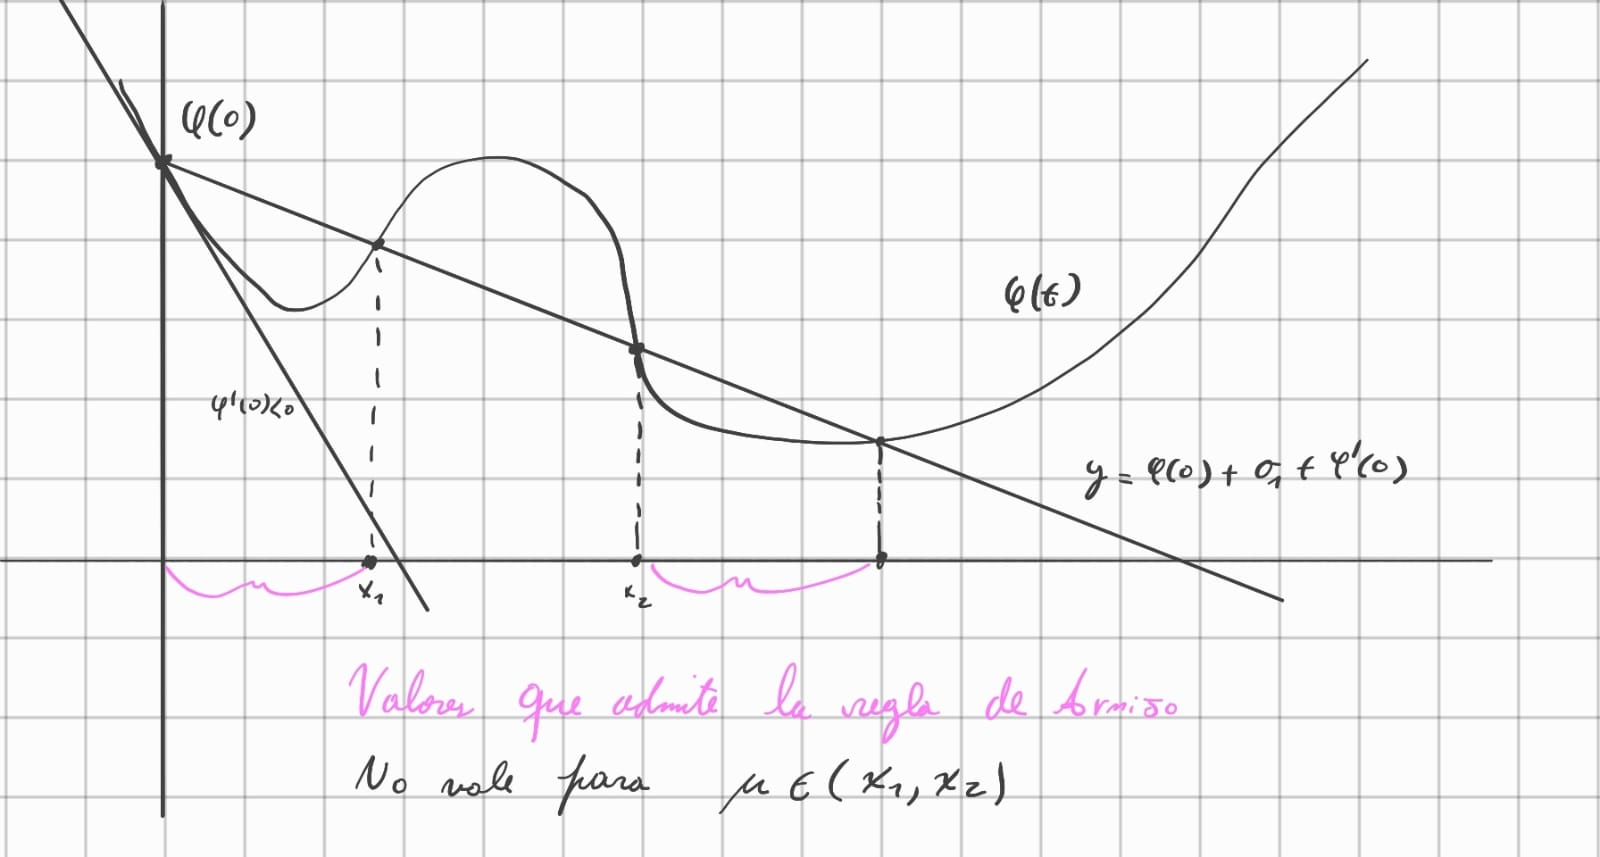
\includegraphics[width=14cm, height=8cm]{media/p2ej1.jpeg}
\end{proof}

\section*{Sección 3.3}
\begin{theorem}{2}
    Considere la función
    \[
        f(x,y) = x - y + 2x^2 + 2xy + y^2.
    \]

    \begin{itemize}
        \item[(a)] Muestre que \(d = (-1,0)\) es una dirección de descenso para \(f\) en \((0,0)\).
              Analizar cuál es el paso óptimo que se puede dar en esa dirección para hacer decrecer el
              valor de \(f\) utilizando búsqueda exacta.

        \item[(b)] Para la dirección de máximo decrecimiento en \((0,0)\) determinar el intervalo
              de paso máximo que se puede dar en esa dirección a partir de \((0,0)\) para hacer decrecer
              el valor de \(f\) utilizando la regla de Armijo con parámetro \(\sigma_1 = 1/4\).
    \end{itemize}
\end{theorem}

\begin{proof}
    Para demostrar (a) notemos que \( f \) es diferenciable y por lo tanto si \( {\nabla f(0,0)}^T \cdot d < 0 \implies d \) es una dirección de descenso. En efecto,
    sea \( d = (-1, 0) \): \begin{align*}
        \nabla{f(x,y)}            & = \begin{pmatrix}
                                          1 + 4x + 2y \\
                                          -1 + 2x + 2y
                                      \end{pmatrix} \\
        \nabla{f(0,0)}            & = \begin{pmatrix}
                                          1 \\
                                          -1
                                      \end{pmatrix} \\
        {\nabla f(0,0)}^T \cdot d & = -1 < 0
    \end{align*}
    Para hallar la longitud del paso óptimo, definimos \( \phi(t) = f((0,0) + t \cdot d) = f(-t, 0) = -t + 2t^2 \), luego \( \phi'(t) = -1 + 4t = 0 \iff t = \frac{1}{4} \) que es la longitud de paso óptima en la dirección \( d \). \\
    Para la parte (b) consideremos la regla de Armijo: \begin{align*}
        f(x + t d) & \leq f(x) + \sigma_1 t {\nabla f(x)}^T d
    \end{align*}
    La dirección de máximo decrecimiento está dada por \( - \nabla f(0,0) = (-1, 1) \), si \( \sigma_1 = \frac{1}{4} \) la regla de Armijo se traduce en: \begin{align*}
        f((0,0) + t \cdot (-1, 1)) & \leq f(0, 0) + \frac{1}{4} t {\nabla f(0,0)}^T \cdot (-1, 1) \\
        f(-t, t)                   & \leq \frac{1}{4} t \cdot (-2)                                \\
        t^2 - 2t                   & \leq -\frac{1}{2} t                                          \\
        t^2 - \frac{3}{2} t        & \leq 0                                                       \\
        t(t - \frac{3}{2})         & \leq 0
    \end{align*}
    Por lo tanto, el intervalo de paso máximo es \( (0, \frac{3}{2}] \).
\end{proof}

\vspace{0.25in}

\begin{theorem}{3}
    Considere la función
    \[
        f(x,y) = 2x^2 + y^2 - 2xy + 2x^3 + x^4.
    \]

    \begin{itemize}
        \item[(a)] Verificar que \(d = (0,1)\) es una dirección de descenso para \(f\) a partir de \((0,-2)\).

        \item[(b)] Para la dirección a partir de \((0,-2)\) considerada en (a), el valor \(t=1\) verifica
              la regla de Armijo con parámetro \(\sigma_1 = 4/5\)?
              ¿Para qué valores de \(\sigma_1\) el valor de longitud de paso \(t=1\) verifica la regla de Armijo?
    \end{itemize}
\end{theorem}

\begin{proof}
    Análogamente al ejercicio anterior, para (a) se tiene que, dado \( d = (0, 1) \): \begin{align*}
        \nabla f(x,y)              & = \begin{pmatrix}
                                           4x - 2y + 6x^2 + 4x^3 \\
                                           2y - 2x
                                       \end{pmatrix} \\
        \nabla f(0,-2)             & = \begin{pmatrix}
                                           4 \\
                                           -4
                                       \end{pmatrix}        \\
        {\nabla f(0,-2)}^T \cdot d & = -4 < 0
    \end{align*}
    Luego, \( d \) es una dirección de descenso para \( f \) en \( (0, -2) \). \\
    Para (b) consideremos la regla de Armijo con \( \sigma_ 1 = \frac{4}{5} \) y \( t = 1 \): \begin{align*}
        f((0,-2) + 1 \cdot (0,1)) & \leq f(0, -2) + \frac{4}{5} \cdot 1 \cdot {\nabla f(0,-2)}^T \cdot (0,1) \\
        f(0, -1)                  & \leq f(0, -2) + \frac{4}{5} \cdot (-4)                                   \\
        1                         & \leq 4 - \frac{16}{5}                                                    \\
        1                         & \leq \frac{4}{5}
    \end{align*}
    Absurdo, luego \( t = 1 \) no verifica la regla de Armijo con \( \sigma_1 = \frac{4}{5} \). \\
    Para hallar los valores de \( \sigma_1 \) para los cuales \( t = 1 \) verifica la regla de Armijo, consideremos: \begin{align*}
        1        & \leq 4 + \sigma_1 \cdot (-4) \\
        \sigma_1 & \leq \frac{3}{4}
    \end{align*}
    Por lo tanto, \( t = 1 \) verifica la regla de Armijo para \( \sigma_1 \in (0, \frac{3}{4}] \).
\end{proof}

\vspace{0.25in}

\begin{theorem}{4}
    Sea \(f\) una función diferenciable tal que \(\nabla f(x) \neq 0\).
    Mostrar que si \(H : \mathbb{R}^n \to \mathbb{R}^{n \times n}\) es una función continua que asigna a
    cada \(x \in \mathbb{R}^n\) una matriz definida positiva \(H(x)\) entonces la dirección
    \[
        d = - H(x) \nabla f(x)
    \]
    es una dirección de descenso para \(f\) en \(x\).
\end{theorem}

\begin{proof}
    Como la matriz  \( H(x) \) es definida positiva y \( \nabla f(x) \neq 0 \) se tiene que \begin{align*}
        {\nabla f(x)}^T \cdot H(x) \cdot \nabla f(x)  & > 0 \\
        -{\nabla f(x)}^T \cdot H(x) \cdot \nabla f(x) & < 0 \\
        {\nabla f(x)}^T \cdot d                       & < 0
    \end{align*}
    y como \( f \) es diferenciable \( d = - H(x) \nabla{f(x)} \) es una dirección de descenso.
\end{proof}

\section*{Sección 3.4}
\begin{theorem}{5}
    Considere la función \( f(x,y) = {(x - 2y)}^2 + x^4 \).
    Calcular la dirección de Newton en el punto \((2,1)\).
    ¿Cumple el valor \(t = 1\) la regla de Armijo con parámetro \(\sigma_1 = 1/5\)?
\end{theorem}

\begin{proof}
    Por definición de dirección de Newton buscamos: \begin{align*}
        \nabla^2 f(2, 1) \cdot d & = - \nabla f(2, 1) \\
    \end{align*}
    Donde \begin{align*}
        \nabla f(x,y)   & = \begin{pmatrix}
                                2(x - 2y) + 4x^3 \\
                                -4(x - 2y)
                            \end{pmatrix} \\
        \nabla f(2,1)   & = \begin{pmatrix}
                                16 \\
                                0
                            \end{pmatrix}   \\
        \nabla^2 f(x,y) & = \begin{pmatrix}
                                2 + 12x^2 & -4 \\
                                -4        & 8
                            \end{pmatrix}   \\
        \nabla^2 f(2,1) & = \begin{pmatrix}
                                50 & -4 \\
                                -4 & 8
                            \end{pmatrix}
    \end{align*}
    Por lo tanto, \begin{align*}
        \begin{pmatrix}
            50 & -4 \\
            -4 & 8
        \end{pmatrix} \cdot d & = \begin{pmatrix}
                                      -16 \\
                                      0
                                  \end{pmatrix} \\
        d                     & = \begin{pmatrix}
                                      -\frac{1}{3} \\
                                      -\frac{1}{6}
                                  \end{pmatrix}
    \end{align*}
    Una vez más, recordemos la regla de Armijo: \begin{align*}
        f(x + t \cdot d) & \leq f(x) + \sigma_1 t {\nabla f(x)}^T \cdot d
    \end{align*}
    En particular,\begin{align*}
        f((2,1) + 1 \cdot (-1/3, -1/6)) & \leq f(2, 1) + \frac{1}{5} \cdot 1 \cdot {\nabla f(2,1)}^T \cdot (-1/3, -1/6) \\
        {\left (\frac{5}{3} \right)}^4  & \leq 16 - \frac{16}{15}                                                       \\
    \end{align*}
    Que es verdadero, luego \( t = 1 \) cumple la regla de Armijo con \( \sigma_1 = \frac{1}{5} \).
\end{proof}
\vspace{0.25in}

\begin{theorem}{6}
    Considere el siguiente método:
    \begin{itemize}
        \item Dado \(x_k\). Calcular \(d_k\) como se indica a continuación.
        \item Hacer \(t = 1\).

              Si \( f(x_k + t d_k) \leq f(x_k) + \tfrac{1}{2} t d_k^T \nabla f(x_k) \) \((*)\) hacer
              \( x_{k+1} = x_k + t d_k \),

              Sino, reemplazar por \(t/2\) hasta que se verifique \((*)\).
    \end{itemize}

    Sea \( f(x,y) = x^2 + y^2 - xy, \; x_0 = (2,0) \).
    \begin{enumerate}
        \item[(a)] Dibuje algunas curvas de nivel de \(f\).
        \item[(b)] Hacer dos iteraciones del método utilizando la dirección de Cauchy. Dibuje los iterados obtenidos en el plano en el cual están las curvas de nivel de \(f\).
        \item[(c)] Resuelva el problema mediante el uso de la dirección de Newton.
    \end{enumerate}
\end{theorem}

\begin{proof}
    \begin{figure}[h!]
        \centering
        \begin{tikzpicture}
            \begin{axis}[
                    title={\(f(x,y) = x^2 + y^2 - xy\)},
                    enlarge x limits,
                    view={0}{90},
                    xlabel=$x$,
                    ylabel=$y$,
                    axis equal image,
                    colormap/viridis,
                    colorbar,                    % show legend for levels
                    colorbar style={title={$f(x,y)$}},
                    axis line style={thick},
                    tick style={thick},
                    grid=both,
                ]
                \addplot3[domain=-3:3,
                    domain y=-3:3,
                    contour gnuplot={levels={0, 2, 4, 6, 8, 10},labels=false},
                    thick,
                    samples=100,
                    samples y=100, ]
                {x^2 + y^2 - x * y};
            \end{axis}
        \end{tikzpicture}
        \caption{(a) Curvas de nivel de \( f(x,y) = x^2 + y^2 - xy \).}
    \end{figure}
    Para (b) consideremos la dirección de Cauchy i.e la dirección de máximo decrecimiento dada por \( - \nabla f(x_k) \). Luego, siguiendo el método propuesto:\begin{align*}
        \nabla f(x, y)                    & = \begin{pmatrix}
                                                  2x - y \\
                                                  2y - x
                                              \end{pmatrix} \\
        \nabla f(2, 0)                    & = \begin{pmatrix}
                                                  4 \\
                                                  -2
                                              \end{pmatrix} \\
        d_0            = - \nabla f(2, 0) & = \begin{pmatrix}
                                                  -4 \\
                                                  2
                                              \end{pmatrix}
    \end{align*}
    Reemplazando en la ecuación: \begin{align*}
        f((2,0) + 1 \cdot (-4, 2)) & \leq^{?} f(2, 0) + \frac{1}{2} \cdot 1 \cdot {\nabla f(2,0)}^T \cdot (-4, 2) \\
        f(-2, 2)                   & \leq^{?} f(2, 0) - 10                                                        \\
        8                          & \leq^{?} -6
    \end{align*}
    que es falso, luego \( t := \frac{1}{2} \) y repetimos: \begin{align*}
        f((2, 0) + \frac{1}{2} \cdot (-4, 2)) & \leq^{?} f(2, 0) + \frac{1}{4} \cdot {\nabla f(2,0)}^T \cdot (-4, 2) \\
        f(0, 1)                               & \leq^{?} f(2, 0) - 5                                                 \\
        1                                     & \leq^{?} -1
    \end{align*}
    que también es falso, luego \( t := \frac{1}{4} \) y de nuevo: \begin{align*}
        f((2, 0) + \frac{1}{4} \cdot (-4, 2)) & \leq^{?} f(2, 0) + \frac{1}{8} \cdot {\nabla f(2,0)}^T \cdot (-4, 2) \\
        \iff f(1, \frac{1}{2})                & \leq^{?} f(2, 0) - \frac{5}{2}                                       \\
        \iff \frac{3}{4}                      & \leq \frac{3}{2}
    \end{align*}
    que es verdadero, entonces definimos \( x_1 = (2, 0) + \frac{1}{4} \cdot (-4, 2) = (1, \frac{1}{2}) \). \\
    Repetimos el proceso para \( x_1 \): \begin{align*}
        \nabla f(1, \frac{1}{2})                   & = \begin{pmatrix}
                                                           \frac{1}{2} \\
                                                           0
                                                       \end{pmatrix} \\
        d_1           = - \nabla f(1, \frac{1}{2}) & = \begin{pmatrix}
                                                           -\frac{1}{2} \\
                                                           0
                                                       \end{pmatrix}
    \end{align*}
    Luego, reinicializando \( t = 1 \): \begin{align*}
        f((1, \frac{1}{2}) + (-\frac{1}{2}, 0)) & \leq^{?} f(1, \frac{1}{2}) + \frac{1}{2} {\nabla f(1, \frac{1}{2})}^T \cdot (-\frac{1}{2}, 0) \\
        \iff f(\frac{1}{2}, \frac{1}{2})        & \leq^{?} f(1, \frac{1}{2}) - \frac{1}{8}                                                      \\
        \iff \frac{1}{4}                        & \leq^{?} \frac{3}{4} - \frac{1}{8}                                                            \\
        \iff \frac{1}{4}                        & \leq \frac{5}{8}
    \end{align*}
    que es verdadero, luego \( x_2 = (1, \frac{1}{2}) + 1 \cdot (-\frac{1}{2}, 0) = (\frac{1}{2}, \frac{1}{2}) \). \\
    Por lo tanto los puntos sobre la curva de nivel quedarían así:

    \begin{figure}[h!]
        \centering
        \begin{tikzpicture}
            \begin{axis}[
                    title={\(f(x,y) = x^2 + y^2 - xy\)},
                    enlarge x limits,
                    view={0}{90},
                    xlabel=$x$,
                    ylabel=$y$,
                    axis equal image,
                    colormap/viridis,
                    colorbar,                    % show legend for levels
                    colorbar style={title={$f(x,y)$}},
                    axis line style={thick},
                    tick style={thick},
                    grid=both,
                ]
                \addplot+[only marks, mark=o] coordinates {(2,0)} node[above right] {$x_0$};
                \addplot+[only marks, mark=o] coordinates {(1,0.5)} node[above right] {$x_1$};
                \addplot+[only marks, mark=o] coordinates {(0.5,0.5)} node[above right] {$x_2$};

                \addplot+[thick] coordinates {(2,0) (1,0.5)};
                \addplot+[thick] coordinates {(1,0.5) (0.5,0.5)};
                % Contour plot
                \addplot3[
                    domain=-3:3,
                    domain y=-3:3,
                    contour gnuplot={levels={0, 2, 4, 6, 8, 10},labels=false},
                    thick,
                    samples=100,
                    samples y=100,
                ]
                {x^2 + y^2 - x * y};
            \end{axis}
        \end{tikzpicture}
        \caption{Curvas de nivel de \( f(x,y) = x^2 + y^2 - xy \) con los puntos \( x_0, x_1, x_2 \) y las direcciones de descenso.}
    \end{figure}

    Por último, para el inciso (c) utilizando la dirección de Newton dada por \( \nabla^2 f(x_k) \cdot d_k = - \nabla f(x_k) \), si consideramos \( x_0 = (2,0) \): \begin{align*}
        \nabla^2 f(x,y)          & = \begin{pmatrix}
                                         2  & -1 \\
                                         -1 & 2
                                     \end{pmatrix}   \\
        \nabla^2 f(2,0)          & = \begin{pmatrix}
                                         2  & -1 \\
                                         -1 & 2
                                     \end{pmatrix}   \\
        \nabla^2 f(2, 0) \cdot d & = - \nabla f(2, 0) \\
    \end{align*}
    Resolviendo el sistema obtenemos \( d = (-2, 0) \implies x_1 = x_0 + d = (0, 0) \) que es el mínimo de la función.
\end{proof}

\section*{Sección 3.6}
\begin{lemma}{Determinante de una matriz}
    Supongamos que \( A \) es una matriz no singular y \( u, v \in \mathbb{R}^n \) no nulos, entonces:\begin{align*}
        \det(A + u v^T) & = \det(A) (1 + v^T A^{-1} u)
    \end{align*}
\end{lemma}

\begin{theorem}{7 Fórmula de Sherman-Morrison}
    Sean \(u, v \in \mathbb{R}^n\) no nulos y \(A \in \mathbb{R}^{n \times n}\) una matriz no singular.
    Sea \( B = A + u v^T \). Demuestre que \(B\) es no singular si y solo si
    \(\sigma = 1 + v^T A^{-1} u \neq 0\). En este caso demuestre que
    \[
        B^{-1} = A^{-1} - \tfrac{1}{\sigma} A^{-1} u v^T A^{-1}.
    \]
\end{theorem}

\begin{proof}
    Para la ida consideremos el contrarrecíproco, si \( 1 + v^T A^{-1} u = 0 \implies \det(A) ( 1 + v^T A^{-1} u) = 0 \implies \det(A + u v^T) = 0 \implies A + u v^T \) es singular por el lema anterior. \\
    Para la vuelta, si \( 1 + v^T A^{-1} u \neq 0 \), \( X = A + uv^T \) e \( Y = A^{-1} - \frac{A^{-1}u v^T A^{-1}}{1+v^T A^{-1}u} \) entonces: \begin{align*}
        XY & = \left(A + uv^T\right) \left( A^{-1} - \frac{A^{-1}u v^T A^{-1}}{1+v^T A^{-1}u} \right)               \\
           & = A A^{-1} + u v^T A^{-1} - \frac{A A^{-1} u v^T A^{-1} + u v^T A^{-1} u v^T A^{-1}}{1 + v^T A^{-1} u} \\
           & = I + u v^T A^{-1} - \frac{u v^T A^{-1} + u v^T A^{-1} u v^T A^{-1}}{1 + v^T A^{-1} u}                 \\
           & = I + u v^T A^{-1} - \frac{u \left(1 + v^T A^{-1} u \right) v^T A^{-1}}{1 + v^T A^{-1} u}              \\
           & = I + u v^T A^{-1} - u v^T A^{-1}                                                                      \\
           & = I
    \end{align*}
    Análogamente se puede probar que \( YX = I \), luego \( Y = X^{-1} \) y por lo tanto \( B \) es no singular y su inversa es la indicada.
\end{proof}
\vspace{0.25in}

\begin{theorem}{8}
    Demostrar que la adaptada BFGS para la inversa cumple:
    Si \(H_k\) es simétrica definida positiva y se tiene que \(s_k^T y_k > 0\)
    entonces \(H_{k+1}\) es simétrica definida positiva.
\end{theorem}

\begin{proof}
    Sea \( \rho_k := \frac{1}{y_k^T s_k} > 0 \), definimos la actualización BFGS para la inversa como: \begin{align*}
        H_{k+1} & = \left(I - \rho_k s_k y_k^T \right) H_k \left(I - \rho_k y_k s_k^T \right) + \rho_k s_k s_k^T
    \end{align*}
    Veamos primero que es simétrica: \begin{align*}
        H_{k+1}^T & = {\left( \left(I - \rho_k s_k y_k^T \right) H_k \left(I - \rho_k y_k s_k^T \right) + \rho_k s_k s_k^T \right)}^T \\
                  & = {\left(I - \rho_k y_k s_k^T \right)}^T H_k^T {\left(I - \rho_k s_k y_k^T \right)}^T + \rho_k s_k s_k^T          \\
                  & = \left(I - \rho_k s_k y_k^T \right) H_k \left(I - \rho_k y_k s_k^T \right) + \rho_k s_k s_k^T                    \\
                  & = H_{k+1}
    \end{align*}
    Usando que si \( A, B, C \) matrices entonces \( {(ABC)}^T = C^T B^T A^T \) y que tanto \( H_k \) como \( \rho_k s_k s_k^T \) son simétricas. \\
    Veamos ahora que está definida positiva, sea \( z \in \R^n \setminus \{ 0 \} \) quiero ver que \( z^T H_{k+1} z > 0 \). Sea \begin{align*}
        w := (I - \rho_k y_k s_k^T) z = z - \rho_k y_k (s_k^T z)
    \end{align*}
    Calculemos \( z^T H_{k+1} z \): \begin{align*}
        z^T H_{k+1} z & = z^T \left( I - \rho_k s_k y_k^T \right) H_k \left(I - \rho_k y_k s_k^T \right) z + z^T \rho_k s_k s_k^T z  \\
                      & = w^T H_k w + {\rho_k (s_k^T z)}^2 \geq 0 \qquad \text{pues } H_k \text{ es definida positiva y } \rho_k > 0
    \end{align*}
    Analicemos si la desigualdad es estricta, si \( z \neq 0 \) entonces: \begin{itemize}
        \item Si \( z^T s_k \neq 0 \implies \rho_k {(z^T s_k)}^2 > 0 \implies z^T H_{k+1} z > 0 \).
        \item Si \( z^T s_k = 0 \implies w = z - \rho_k y_k (s_k^T z) = z \implies z^T H_{k+1} z = z^T H_k z > 0 \) pues \( z \neq 0 \) y \( H_k \) es definida positiva.
    \end{itemize}
\end{proof}
\vspace{0.25in}

\begin{theorem}{9}
    Considere el método de Quasi-Newton con fórmula adaptada secante DFP de rango 2
    con búsqueda lineal exacta y matriz inicial \(H_0\) definida positiva.
    Demuestre que \(y_k^T s_k > 0\) para todo \(k\).
    Ídem si se utiliza la búsqueda de Wolfe.
\end{theorem}

\begin{proof}
    Recordemos que \( s_k = x_{k+1} - x_k \) e \( y_k = \nabla f(x_{k+1}) - \nabla f(x_k) \). Si la búsqueda lineal es exacta, definamos: \begin{itemize}
        \item \( g_k = \nabla f(x_k) \).
        \item \( p_k = - H_k g_k \) la dirección de descenso.
        \item \( s_k = x_{k+1} - x_k = t_k p_k \) con \( t_k \) la longitud del paso óptimo.
        \item \( y_k = g_{k+1} - g_k \).
        \item \( \phi_k(t) = f(x_k + t p_k) \).
    \end{itemize}
    Notemos que \( -g_k^T H_k g_k < 0 \). Por lo tanto existe un \( t_k \) que minimiza la función. Luego, \begin{align*}
        \phi_k'(t_k) & = 0 \qquad \text{ y } \qquad g_{k+1}^T p_k = 0                                       \\
                     & \implies y_k^T s_k = {(g_{k+1} - g_k)}^T (x_{k+1} - x_k) = g_{k+1}^T s_k - g_k^T s_k \\
    \end{align*}
    Como \( s_k = t_k p_k \) y \( g_{k+1}^T p_k = 0 \) se tiene que: \begin{align*}
        g_{k+1}^T s_k & = t_k g_{k+1}^T p_k = 0                                                                                     \\
                      & \implies y_k^T s_k = - g_k^T s_k = - t_k g_k^T p_k > 0 \qquad \text{pues } t_k > 0 \text{ y } g_k^T p_k < 0
    \end{align*}
    Si la búsqueda es de Wolfe, se tiene que dado \( \sigma_2 \in (0, 1) \): \begin{align*}
        g_{k+1}^T p_k \geq \sigma_2 g_k^T p_k
    \end{align*}
    Nuevamente \( s_k = t_k p_k \) así: \begin{align*}
        y_k^T s_k = {(g_{k+1} - g_k)}^T  s_k = t_k (g_{k+1}^T p_k - g_k^T p_k)
    \end{align*}
    Aplicando la desigualdad en el primer termino se obtiene: \begin{align*}
        g_{k+1}^T p_k - g_k^T p_k \geq \sigma_2 g_k^T p_k - g_k^T p_k = (\sigma_2 - 1) g_k^T p_k
    \end{align*}
    Entonces, \begin{align*}
        y_k^T s_k & \geq t_k (\sigma_2 - 1) g_k^T p_k > 0 \qquad \text{pues } t_k > 0, \; \sigma_2 - 1 < 0 \text{ y } g_k^T p_k < 0
    \end{align*}
\end{proof}

\vspace{0.25in}

\end{document}